\scanpage{153}
\figure{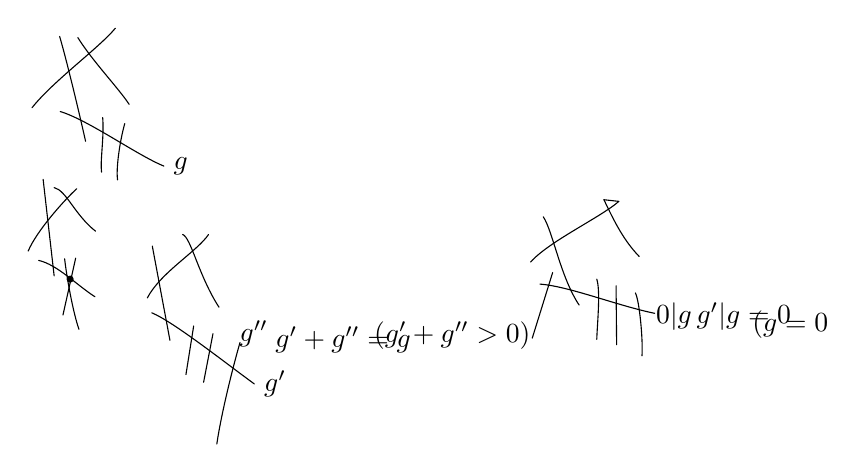
\begin{tikzpicture}[x=.007cm,y=-.007cm,line cap=round]
\draw (196,340).. controls (235,291) and (316,233)..(347,196);
\draw (246,211).. controls (260,259) and (282,352)..(293,401);
\draw (279,213).. controls (305,255) and (353,305)..(372,334);
\draw (247,347).. controls (299,363) and (386,426)..(435,446) node[right] {$g$};
\draw (324,358).. controls (327,392) and (319,438)..(322,457);
\draw (364,369).. controls (355,401) and (348,450)..(351,471);
\draw (189,600).. controls (204,564) and (254,508)..(277,487);
\draw (216,470)--(236,645);
\draw (236,485).. controls (258,490) and (273,534)..(311,564);
\draw (208,617).. controls (242,625) and (276,661)..(310,683);
\draw (255,614).. controls (259,650) and (271,714)..(281,742);
\draw (275,613)--(252,716);
\fill (265,651) circle[radius=.045cm];
\draw (405,685).. controls (429,639) and (495,601)..(516,570);
\draw (414,591)--(446,762);
\draw (469,570).. controls (484,575) and (498,645)..(535,702);
\draw (413,712).. controls (452,728) and (548,804)..(599,841) node[right] {$g'$};
\draw (489,736)--(475,824); \draw (524,750)--(507,838);
\draw (573,766).. controls (560,811) and (539,895)..(531,950);
\node at (598,750) {$g''$};
\node at (760,761) {$g'+g''=g$};
\node at (958,754) {$(g'+g''>0)$};
\draw (1100,620).. controls (1134,582) and (1227,539)..(1260,510);
\draw (1123,538).. controls (1140,563) and (1154,647)..(1188,698);
\draw (1233,507).. controls (1252,547) and (1269,581)..(1297,610);
\draw (1233,507)--(1260,510);
\draw (1117,660).. controls (1170,664) and (1257,699)..(1325,713);
\draw (1140,639)--(1103,758);
\draw (1220,651).. controls (1227,673) and (1221,730)..(1220,760);
\draw (1255,663)--(1256,770);
\draw (1290,676).. controls (1297,689) and (1304,758)..(1302,790);
\node[anchor=west] at (1310,719) {$\deleted{\unsure{0|g}}\,\unsure{g'|g}=0$};
\node at (1571,733) {$(g=0$};
\end{tikzpicture}}
\[
\sum_{g_i\geq1}(3g_i-3+\nu_i\deleted{\unsure{-1|1}})
+\sum_{g_i=1}(1\underbrace{+\nu_i-1}_{3g_i-3+\nu_i})
+\sum_{\substack{g_i=0\\\nu_i\geq3}}\deleted{\unsure{\substack{\sup(0,\\\sup(0,}}}\underset{3g_i-3+\nu_i}{\nu_i-3}
\]
$\nu_i=$ nb des pts \deleted{\unsure{multiples}} \inserted{\unsure{$P_{\alpha}$|dbls|doubles}} sur $C_i$
\[
3\sum g_i-3c_0+\sum\nu_i\overset{\inserted{\lambda}}{+}
\boxed{\sum_{\substack{g_i=0\\\nu_i\unsure{\leq|=}2}}3-\nu_i}
\]
$\lambda=$ nb des \deleted{\unsure{courbes|composantes}} $C_i$ de genre $0$, avec $\nu_i=2$ (\unsure{minimum})

\figure{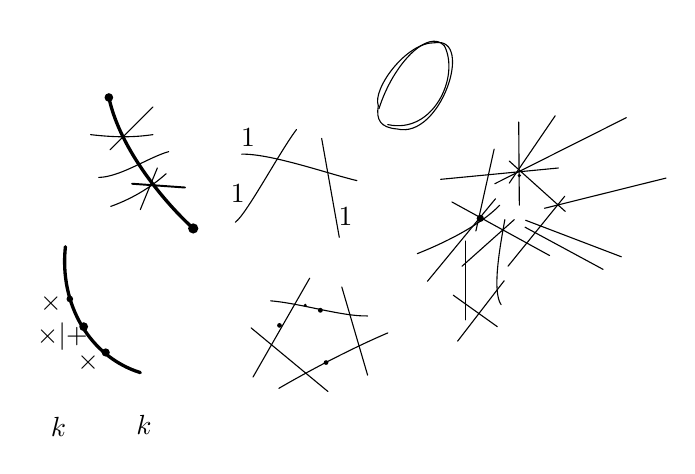
\begin{tikzpicture}[x=.008cm,y=-.008cm,line cap=round]
\draw (649,1454).. controls (639,1428) and (693,1353)..(739,1354)
.. controls (802,1344) and (748,1508)..(679,1491).. controls (653,1489) and (645,1477)..(649,1454);
\draw (650,1459).. controls (673,1386) and (729,1331)..(754,1359)
.. controls (779,1408) and (736,1500)..(664,1484);
\draw[line width=1.2pt] (221,1441).. controls (239,1525) and (312,1610)..(355,1649);
\fill (221,1441) circle[radius=.055cm]; \fill (355,1649) circle[radius=.065cm];
\draw (192,1500).. controls (235,1505) and (263,1504)..(291,1500);
\draw (223,1524)--(291,1456);
\draw (205,1568).. controls (240,1567) and (284,1536)..(316,1527);
\draw (224,1614).. controls (263,1600) and (292,1580)..(312,1562);
\draw[line width=.7pt] (258,1578)--(342,1584); \draw (271,1619)--(298,1553);
\draw (422,1639).. controls (440,1626) and (493,1526)..(519,1492);
\draw (432,1531).. controls (479,1530) and (572,1563)..(615,1573);
\draw (559,1506)--(587,1663);
\node at (442,1504) {$1$}; \node at (426,1593) {$1$}; \node at (597,1630) {$1$};
\draw[line width=1.2pt] (152,1678).. controls (142,1770) and (191,1853)..(271,1878);
\fill (159,1761) circle[radius=.042cm]; \fill (181,1805) circle[radius=.056cm]; \fill (216,1846) circle[radius=.052cm];
\node at (129,1768) {$\times$}; \node at (147,1820) {$\unsure{\times|+}$}; \node at (188,1862) {$\times$};
\node at (141,1964) {$k$}; \node at (277,1961) {$k$};
\draw (478,1764).. controls (526,1768) and (592,1789)..(632,1788);
\draw (450,1885)--(540,1728); \draw (591,1742)--(632,1882);
\draw (447,1807)--(569,1908);
\draw (491,1903).. controls (546,1871) and (610,1838)..(664,1815);
\fill (492,1803) circle[radius=.03cm]; \fill (533,1771) circle[radius=.021cm];
\fill (557,1779) circle[radius=.031cm]; \fill (566,1862) circle[radius=.03cm];
\draw (748,1571)--(935,1553); \draw (872,1480)--(873,1612);
\draw (834,1578)--(1043,1473); \draw (857,1577)--(930,1470);
\draw (857,1542)--(946,1622); \draw (913,1617)--(1106,1569);
\draw (833,1523)--(804,1653); \draw (711,1689).. controls (754,1672) and (811,1644)..(842,1612);
\draw (766,1607)--(921,1692); \draw (727,1733)--(835,1602);
\draw (782,1709)--(865,1635); \draw (850,1635).. controls (841,1684) and (830,1749)..(844,1770);
\draw (855,1709)--(945,1598); \draw (883,1636)--(1035,1694); \draw (882,1647)--(1006,1714);
\draw (788,1669)--(788,1794); \draw (768,1755)--(838,1805); \draw (775,1828)--(849,1732);
\fill (811,1633) circle[radius=.046cm]; \fill (873,1565) circle[radius=.023cm];
\end{tikzpicture}}
\margin{[tout cycle est formé \unsure{exclusivemt|exclusivement} de courbes rationnelles, et \deleted{\unsure{est de longueur}} \inserted{\unsure{un cycle}} minimum est de longueur \unsure{au|n}}%
\[
\sum g_i=g-\overset{\substack{\text{\unsure{nb des cycles}}\\\text{\unsure{combin.|combinatoires}}}}{\rho}.
\]
\[
3g-
\]
% archive sheet number: 152
